\Chapter{Koordináta-rendszerek}

\section{Négyzet}

Négyzetrács esetében egy derékszögű koordináta-rendszer használata a legkézenfekvőbb. 
\newline
\newline A derékszögű koordináta rendszert két egymásra merőleges számegyenes alkotja. Az egyeneseket koordináta tengelyeknek, metszéspontjukat kezdőpontnak, origónak nevezzük. Az origóhoz mindkét számegyenesen a $0$-t rendeljük hozzá. A „vízszintes” tengely az $x$ (abszcissza) tengely, a „függőleges” az $y$ (ordináta) tengely.
\newline
\newline A koordináta rendszer segítségével a sík bármely $P$ pontjának a helyzete két jelzőszám (koordináta) segítségével egyértelműen meghatározható. A pont helyzetét a két tengelytől mért előjeles távolságával határozzuk meg. A pontnak a tengelyektől mért előjeles távolságai a pont koordinátái (jelzőszámai). Az előjelek a számegyenesek segítségével adhatók meg. A jelzőszámokat, a pont neve után zárójelben adjuk meg: $P(x;y)$.

\section{Hexagon}

A hexagonok hat oldalú poligonok. A szabályos hatszögnek minden oldala egyenlő hosszúságú és belső szögei is egyező fokúak. A szakdolgozatomban csak szabályos hatszögekkel fogok foglalkozni. 
\newline
\newline Egy hexagonnak hat oldala van. Minden oldalon két hexagon osztozik. Egy hexagonoknak hat csúcsa van, minden csúcson 3 hexagon osztozik.
\newline
\newline A hexagonháló esetében többfajta megközelítés is szóbajöhet, hogyan kezeljük őket koordináta rendszerben, most ezek közül fogok néhányat ismertetni. 

\subsection{Eltolásos koordináta-rendszer (Offset coordinates)}

A leggyakoribb megközelítés az eltolásos módszer, ami kisebb eltérésektől eltekintve gyakorlatilag megegyezik a négyzet koordináta-rendszerrel. 
\newline
\newline\newline

\begin{figure}[h]
\centering
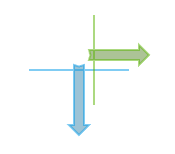
\includegraphics[scale=0.5]{kepek/img41.png}
\caption{Az eltolásos koordináta-rendszerben a tengelyek elhelyezkedése.}
\label{fig:img41}
\end{figure}

\noindent A négyzethálóval is elérhetünk a hexagonhálóhoz hasonló hatást, ha a négyzethálóban minden páros/páratlan sort/oszlopot eltolunk.

\begin{figure}[h]
\centering
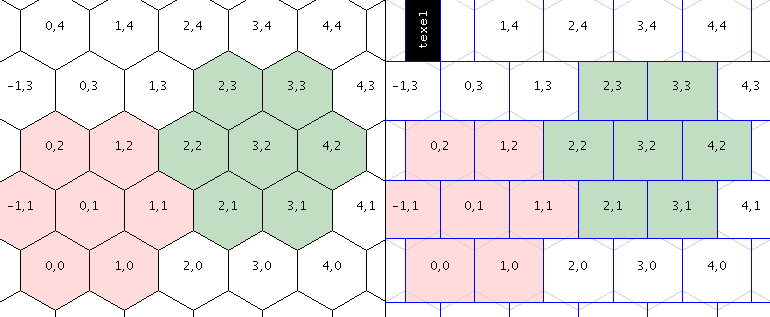
\includegraphics[scale=0.5]{kepek/img42.png}
\caption{Hexagon rács az eltolt négyzetrácshoz viszonyítva}
\label{fig:img42}
\end{figure}

Eltolható a páros és a páratlan oszlop/sor is. Mivel kétféleképpen is állhatnak a hexagonok, ezért 4 fajta variáció érhető el összesen.
\newline
\newline A négyzet koordináta-rendszerhez hasonlóan itt is a hálónk egyik sarka lesz a kezdő pont (origó) amihez viszonyítva számozzuk majd a sorokat és oszlopokat.
\newline
\newline Az eltolásos koordináta-rendszernek az egyik hátránya, hogy a kettőből az egyik tengelye mentén nem egyenesen halad a hexagonok az eltolás miatt, ezáltal bonyolítva a dolgokat. A további rendszerek ezt a problémát orvosolják, viszont ott más problémák merülnek fel.		

\subsection{Kocka koordináta-rendszer (Cube coordinates)}

Egy másik fajta megközelítésből nézzük a hexagon hálókat, akkor láthatjuk, hogy három elsődleges tengelye van, nem úgy mint a korábbi koordináta-rendszereknek. 

\begin{figure}[h]
\centering
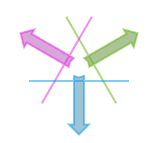
\includegraphics[scale=0.3]{kepek/img43.png}
\caption{A kocka koordináta rendszerben a tengelyek elhelyezkedése.}
\label{fig:img43}
\end{figure}

\noindent Ahhoz, hogy megértsük a kocka koordináta-rendszert képzeljünk el egy kockarácsot és vágjunk ki belőle egy átlós síkot az $x + y + z = 0$ mentén. Ez fogja majd a hexagon rácson használt algoritmusokat egyszerűbbé tenni. Azáltal, hogy használhatjuk a Descartes-féle koordináta-rendszerben való műveleteket: hozzáadás a koordinátákhoz, kivonás a koordinátákból, szorzás vagy osztás skalárral, távolság számítás.
\newline
\newline Egy szemléletesebb példaként vizsgáljuk meg a Q*bert nevű játékot.

\begin{figure}[h]
\centering
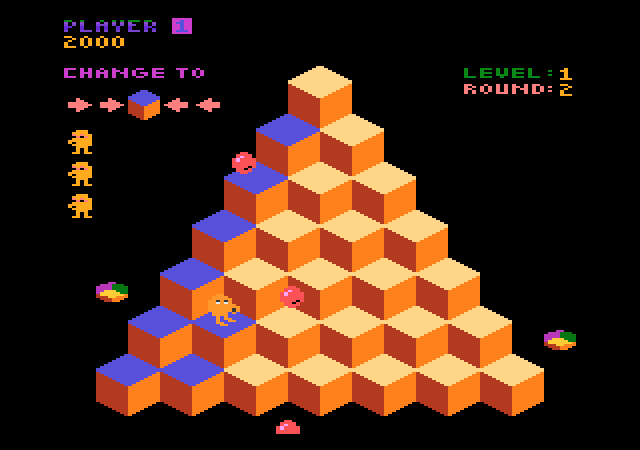
\includegraphics[scale=0.3]{kepek/img44.png}
\caption{A Q*bert című játék.}
\label{fig:img44}
\end{figure}

\noindent A játék egy $28$ kockából álló piramis szerű játékmezőn zajlik (Ilyen alakzatot kapunk, ha végrehajtjuk a fent írtakat.). A játékos Q*bert-et (narancssárga karakter) irányítja, aki, ha ráugrik egy kockára akkor átszínezi azt.
\newline
\newline Ha jobban megfigyeljük az ábrát, akkor láthatjuk, hogy a kockák valójában hexagonok, ha 2D-ben rendereljük, ha így nézzük, akkor Q*bert 6 különböző irányba is léphet. Ez azt jelenti, hogy a párhuzamosan lévő oldalakra merőlegesen helyezünk tengelyeket, akkor hármat tudunk elhelyezni 120 fokonként.

\begin{itemize}
\item Minden hexagonnak 3 koordinátája van. 
\item Mindegyik tengely egy egyenes vonalnak felel meg a hexagon hálón.
\item Minden irány a hexagonon másik két iránynak a kombinációja a kocka koordináta-rendszeren. Például, ha a 4.5. ábrán felfelé szeretnénk mozogni, akkor az a {\color{magenta} $+y$} és {\color{blue} $-z$} között fekszik, ezért minden lépésnél ami felfelé történik hozzá kell adnunk 1-et az {\color{magenta} $y$}-hoz és el kell vennünk 1-et a {\color{blue} $z$}-ből. 

\begin{figure}[h]
\centering
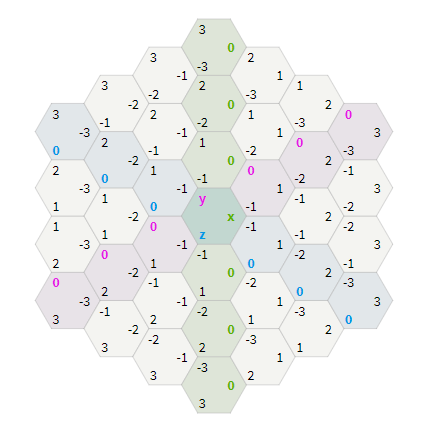
\includegraphics[scale=0.3]{kepek/img45.png}
\caption{A kocka koordináta-rendszer.}
\label{fig:img45}
\end{figure}

\end{itemize}

\noindent Ez azért történik mert minden egyes mező koordinátájának az összege $0$ kell, hogy legyen ($x + y + z = 0$). Ez azt is jelenti, hogy a harmadik tengely bizonyos esetekben redundáns is lehet, például amikor meghatározzuk, hogy az egyes mezők hol jelenjenek meg a képernyőn, ugyanakkor olyan esetekben mint az útkereső vagy a távolság számító algoritmusok az előnye egyértelműen látszik. 

\subsection{Tengely koordináta-rendszer (Axial coordinates)}

Tengely koordináta-rendszer csak kettő koordinátát használ a kocka koordináta-rendszer három koordinátája közül. Mivel a kocka koordináta-rendszernél volt az a megkötés, hogy $x + y + z = 0$, és ahogy már a kocka koordináta-rendszernél már leírtam a harmadik koordináta redundáns.  A tengelyes koordináta-rendszer használható tárolásra és megjelenítésére és mivel az $x + y + z = 0$ egyenlet alapján kiszámítható a harmadik koordináta ezért a számításokhoz is könnyen használható.

\begin{figure}[h]
\centering
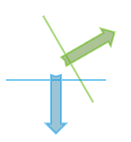
\includegraphics[scale=0.5]{kepek/img46.png}
\caption{A tengelyes koordináta rendszerben a tengelyek elhelyezkedése.}
\label{fig:img46}
\end{figure}

\noindent Az előnye ennek a rendszernek az eltolásoshoz képest, hogy az algoritmusok egyszerűbbek. A hátránya ennek a rendszernek a téglalap alakú térképek esetén való tárolás. 
